\begin{figure}
\centering
    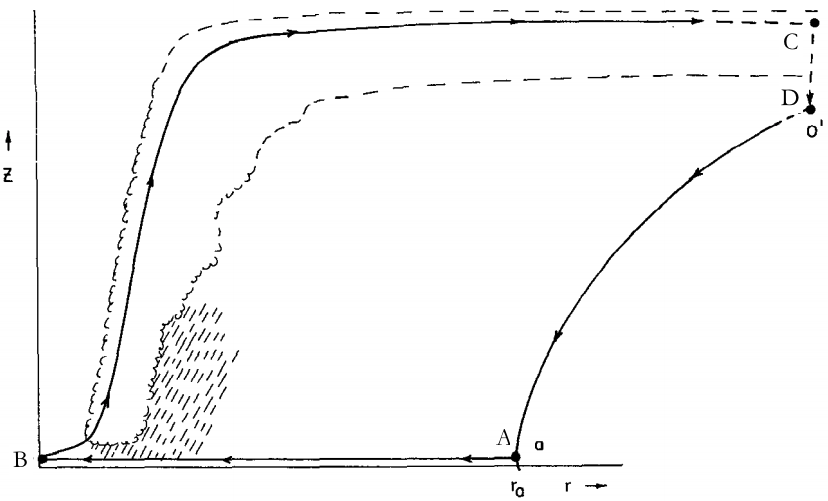
\includegraphics[width=\linewidth]{images/hurricane-carnot.png}\\
    \textit{Figure 1 from~\cite{emanuel1991theory}. }
    \caption{An idealised Carnot cycle where air parcels travel clockwise;
            travelling inwards into the eye-wall extracting thermal energy
            from the sea; adiabatically thrust up into the stratosphere
            at the eye-wall and out to some some subsidence point. }
            \label{fig:hurricane-carnot}

\end{figure}


Enthalpy is acquired from the sea surface,
and entropy from the dissipation of kinetic energy,
 as the air travels isothermally towards the eyewall.
 At the eyewall the air rises moist adiabatically
 to the lower stratosphere and out to some distance from the storm.
 In a simplified model it then subsides
 approximately isothermally at first, albeit with some loss through radiation.
 The final descent is approximately moist adiabatic~\ref{emanuel2018progress}.

This is nearly an ideal carnot cycle, this converts heat energy of the sea surface into
mechanical energy of the winds, doing the majority of the work against the sea surface.

\begin{equation}
\left|\mathbf{V}_{s}\right|^{2}=\frac{C_{k}}{C_{D}} \frac{T_{s}-T_{o}}{T_{o}}\left(k_{0}^{*}-k\right)
\tag{PI}
\label{eq:PI}
\end{equation}

where $C_d$ is the surface drag coefficient $C_k$ is the dimensionaless
surface exchange coefficient for enthalpy.

$T_s$ is the sea surface temperature, $T_o$ is the temperature of the
lower stratosphere at the end of the moist adiabatic rise.

\begin{equation}
k \equiv c_{p} T+L_{v} q
\end{equation}

$c_p$ is the heat capacity at constant pressure and $L_{v}$ is the latent heat
of vaporisation. $k_{0}^{*}$ is the saturation enthalpy at the sea surface.
